\documentclass[12pt,a4paper,ngerman]{report}
\usepackage{graphicx}
\usepackage{ifpdf}
\ifpdf
   % put here packages only for the PDF:
   \DeclareGraphicsExtensions{.pdf,.png,.jpg,.mps}
   \usepackage{hyperref}
\else
   % put here packages only for the DVI:
\fi

% put all the other packages here:
\usepackage{amsmath}
\usepackage{amsthm}
\usepackage{algorithm}
\usepackage{varwidth}
\usepackage[noend]{algpseudocode}
\usepackage{tikz}
\usetikzlibrary{shapes,shapes.geometric,arrows,fit,calc,positioning,automata}

\newtheorem{theorem}{Satz}
\newtheorem{bem}{Bemerkung}

\usepackage{style}
\algblockdefx[Foreach]{Foreach}{EndForeach}[1]{\textbf{foreach} #1 \textbf{do}}{\textbf{end foreach}}
\begin{document}

%% hsrm logo in the background, from the beamer theme
\AddToShipoutPicture*{\includegraphics[width=\paperwidth]{slides/background.pdf}}

\title{Implementierung des „Generalized Asymmetric Partition Crossover“
als Teil eines evolutionären Algorithmus in einem parallelisierten
Erlang-System}

\author{Jan Niklas Böhm\\ Fachbereich DCSM\\ \texttt{mail@jnboehm.com}\\
            \and
        Jens Nazarenus\\ Fachbereich DCSM\\ \texttt{me@jens-na.de}}


\maketitle

\chapter*{Vorwort}
Diese Ausarbeitung entstand im Rahmen eines Studienprojektes im Wahlpflichtmodul
„Graphentheorie und Graphenalgorithmen“ an der Hochschule RheinMain.


% if we want to shorten the toc
% \setcounter{tocdepth}{0}
\tableofcontents
\listoffigures
\listoftables

\input{./tex/intro.tex}
\chapter{Einführung}
\section{„Asymmetrisches Traveling Salesman“ (ATSP) Problem}
Das Problem des Handlungsreisenden ist ein
\textbf{NP-hartes}\cite{exakte_algo} kombinatorisches Problem, bei dem versucht wird in
einem vollständigen, \textit{gerichteten} Graphen die kürzeste Rundreise zu
finden. Jeder Knoten muss dabei genau einmal besucht werden.

\section{Komplexität}
Um die kürzeste Rundreise in einem vollständigen, gerichteten Graphen zu
ermitteln, kann man die Kosten für jede mögliche Rundreise berechnen,
um den optimalen Weg zu finden. Es gibt $(n-1)!$
Rundreisen, die zu untersuchen sind\cite{pursuit}. Dies bedeutet, dass 
der Rechenaufwand für das Problem 
des Handlungsreisenden exponentiell mit der Anzahl der Knoten im Graphen
wächst, dadurch $\in 
\mathcal{O}(n!)$ und somit auch~$\in$~\textbf{NP}, falls 
\textbf{P} $\neq$ \textbf{NP}.
\begin{bem}
Die Anzahl der möglichen Rundreisen bei einer Knotenanzahl von $4$ wären also
$(4-1)! = 1 \cdot 2 \cdot 3 = 6$. Wählen wir $n = 20$ würde die
Anzahl der möglichen Rundreisen bereits $(20-1)! =
121645100408832000$ betragen.
\end{bem}

\section{Lösungsidee}
In der Praxis werden heutzutage trotz allem „gute“ Lösungen benötigt.
Eine direkte Berechnung der besten Lösung ist aber für eine große
Knotenanzahl nicht praxistauglich. In dieser Ausarbeitung wird
vorgestellt wie man gute Lösungen mit einem sogenannten „evolutionären
Algorithmus“ heuristisch findet. Ebenfalls wird eine in der
Programmiersprache Erlang entwickelte Implementierung des Algorithmus 
beschrieben.

In der Ausarbeitung wird beschrieben wie der Rekombinationsoperator
„Generalized Asymmetric Partition Crossover“ funktioniert und
implementiert wurde.
Ein weiterer notwendiger Teil der Implementierung ist die Optimierung
von Rundreisen mit einem modifiziertem „3-opt“-Verfahren.

\chapter{Generalized Asymmetric Partition Crossover}

\section{Einleitung}
Der „Generalized Asymmetric Partition Crossover“ (GAPX) ist ein
Rekombinationsoperator, der als Teil eines evolutionären Algorithmus
verwendet werden kann. Aufgabe einer Rekombination beim ATSP ist es aus
zwei gegebenen Rundreisen $G_1$, $G_2$ ein Kind (auch Offspring genannt)
$G_o$ zu erzeugen.


\begin{algorithm}
\caption{Crossover in einem EA}\label{alg:crossover_ea}
\begin{algorithmic}[1]
\Procedure{Crossover}{$G_1,G_2$}\Comment{}
\State $G_o\gets gapx(G_1,G_2)$\Comment{In 2.2 beschrieben}
\State \textbf{return} $G_o$
\EndProcedure
\end{algorithmic}
\end{algorithm}
GAPX versucht durch ein bestimmtes Verfahren die beiden Rundreisen zu
partitionieren und daraus das neue Kind $G_o$ zu erzeugen.


\section{Funktionsweise}
Seien $G_1$ und $G_2$ beliebige Rundreisen, beide erzeugt aus einem
vollständigen Graphen $G_c$. Zunächst werden $G_1$ und $G_2$ in einem
gemeinsamen Graphen $G_u$ zusammengeführt. Den Graph $G_u = G_1 \cup
G_2$ nennen wir auch Vereinigungsgraph von $G_1$ und $G_2$.
\newpage
%% Bild mergen von G1, G2
\begin{figure}[hb]
\centering
\renewcommand{\arraystretch}{3.5}
\begin{tabular}{ c c c }
$G_1$ & $G_2$ & $G_u$ \\
\resizebox{90pt}{90pt}{

  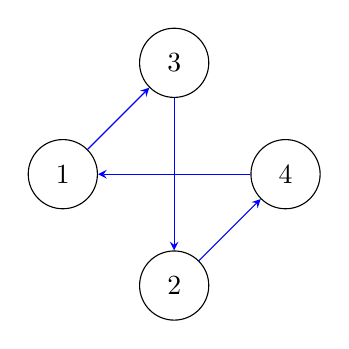
\begin{tikzpicture}[%
    >=stealth,
    node distance=2cm,
    on grid,
    auto
  ]
  \node[state] (1){1};
  \node[state] (3) [above right of=1]{3};
  \node[state] (2) [below right of=1]{2};
  \node[state] (4) [below right of=3]{4};
  
  \path[->] (1) edge [blue, bend left=0] node  {} (3);
  \path[->] (3) edge [blue, bend left=0] node  {} (2);
  \path[->] (2) edge [blue, bend left=0] node  {} (4);
  \path[->] (4) edge [blue, bend left=0] node  {} (1);
  
  \end{tikzpicture}
} 

& 

\resizebox{90pt}{90pt}{

  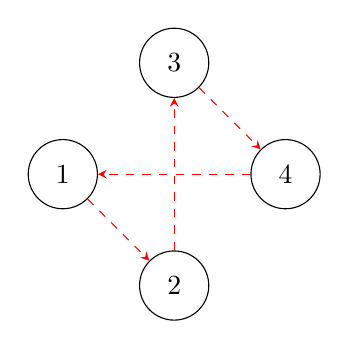
\begin{tikzpicture}[%
    >=stealth,
    node distance=2cm,
    on grid,
    auto
  ]
  \node[state] (1){1};
  \node[state] (3) [above right of=1]{3};
  \node[state] (2) [below right of=1]{2};
  \node[state] (4) [below right of=3]{4};

  \path[->] (1) edge [red, dashed, left=0] node  {} (2);
  \path[->] (2) edge [red, dashed, left=0] node  {} (3);
  \path[->] (3) edge [red, dashed, left=0] node  {} (4);
  \path[->] (4) edge [red, dashed, left=0] node  {} (1);

  \end{tikzpicture}
} 

&

\resizebox{90pt}{90pt}{

  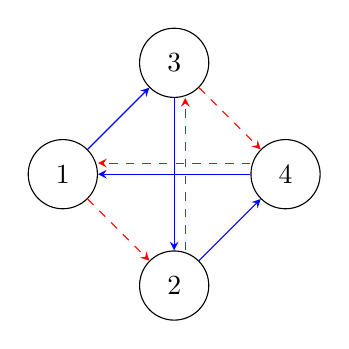
\begin{tikzpicture}[%
    >=stealth,
    node distance=2cm,
    on grid,
    auto
  ]
  \node[state] (1){1};
  \node[state] (3) [above right of=1]{3};
  \node[state] (2) [below right of=1]{2};
  \node[state] (4) [below right of=3]{4};

  \path[->] (1) edge [blue, bend left=0] node  {} (3);
  \path[->] (3) edge [blue, bend left=0] node  {} (2);
  \path[->] (2) edge [blue, bend left=0] node  {} (4);
  \path[->] (4) edge [blue, bend left=0] node  {} (1);

  \path[->] (1) edge [red, dashed, left=0] node  {} (2);
  \path[->] ([xshift=0.4em] 2.north) edge 
      [red, dashed, left=0] node  {} ([xshift=0.4em] 3.south);
  \path[->] (3) edge [red, dashed, left=0] node  {} (4);
  \path[->] ([yshift=0.4em] 4.west) edge 
      [red, dashed, left=0] node  {} ([yshift=0.4em] 1.east);

  \end{tikzpicture}
} 
\end{tabular}
\renewcommand{\arraystretch}{1}
\caption[Beispiel einer Zusammenlegung von Graphen]{
Beispiel für das Zusammenführen der Graphen $G_1$ und $G_2$ zu
dem neuen Graphen $G_u$ anhand zwei Rundreisen mit je vier Knoten.
}
\end{figure}
%%\begin{bem}
%%  Streng genommen ist $G_u$ ein Multigraph, da doppelte Kanten zwischen
%%  Knoten existieren können, jedoch hat dies die Implementierung nicht
%%  eingeschränkt, da ein „normaler Graph“ eine Spezielform eines
%%  Multigraphen ist.
%%\end{bem}
Nach der Zusammenführung der beiden Graphen in $G_u$ muss für alle
Knoten $v$ aus $G_u$ bei der die Bedingung $deg(v) = 4$ erfüllt ist ein
sogenannter Ghost-Knoten $v'$ eingeführt werden. Zusätzlich muss eine
Kante mit dem Gewicht $0$ zwischen $v$ und $v'$ eingefügt werden. 
Der Graph $G_u$ mit eingefügten Ghost-Knoten an den entsprechenden Stellen kennzeichnen wir als $G_u'$.
\begin{figure}[hb]
\centering
\begin{tabular}{ c c }
\resizebox{120pt}{170pt}{
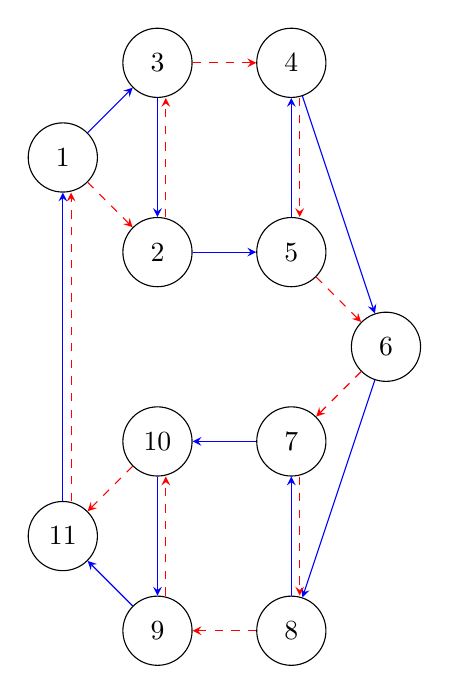
\begin{tikzpicture}[%
>=stealth,
node distance=1.7cm,
on grid
]
\node[state] (1)              {1};


\node[state] (3) [above right of=1]             {3};
\node[state] (2) [below right of=1]            {2};
\node[state] (4) [right of=3]             {4};
\node[state] (5) [right of=2]             {5};

\node[state] (6) [below right of=5] {6};

\node[state] (7) [below left of=6] {7};
\node[state] (10) [left of=7] {10};

\node[state] (11) [below left of=10] {11};

\node[state] (9) [below right of=11] {9};
\node[state] (8) [right of=9] {8};

% solid: parent 1
\path[->] (1) edge [blue, bend left=0] node  {} (3);
\path[->] (3) edge [blue, bend left=0] node  {} (2);
\path[->] (2) edge [blue, bend left=0] node  {} (5);
\path[->] (5) edge [blue, bend left=0] node  {} (4);
\path[->] (4) edge [blue, bend left=0] node  {} (6);
\path[->] (6) edge [blue, bend left=0] node  {} (8);
\path[->] (8) edge [blue, bend left=0] node  {} (7);
\path[->] (7) edge [blue, bend left=0] node  {} (10);
\path[->] (10) edge [blue, bend left=0] node  {} (9);
\path[->] (9) edge [blue, bend left=0] node  {} (11);
\path[->] (11) edge [blue, bend left=0] node  {} (1);

% dashed: parent 2
\path[->] (1) edge [bend left=0, dashed, red] node {} (2);
\path[->] ([xshift=0.7ex] 2.north) edge [red, dashed] node {}
         ([xshift=0.7ex] 3.south);
\path[->] (3) edge [red, dashed] node {}
         (4);
\path[->] ([xshift=0.7ex] 4.south) edge [red, dashed] node {}
         ([xshift=0.7ex] 5.north);
\path[->] (5) edge [red, dashed] node {}
         (6);
\path[->] (6) edge [red, dashed] node {}
         (7);
\path[->] ([xshift=0.7ex] 7.south) edge [red, dashed] node {}
         ([xshift=0.7ex] 8.north);
\path[->] (8) edge [red, dashed] node {}
         (9);
\path[->] ([xshift=0.7ex] 9.north) edge [red, dashed] node {}
         ([xshift=0.7ex] 10.south);
\path[->] (10) edge [red, dashed] node {}
         (11);
\path[->] ([xshift=0.7ex] 11.north) edge [red, dashed] node {}
         ([xshift=0.7ex] 1.south);
\end{tikzpicture}
}

&
\resizebox{120pt}{170pt}{
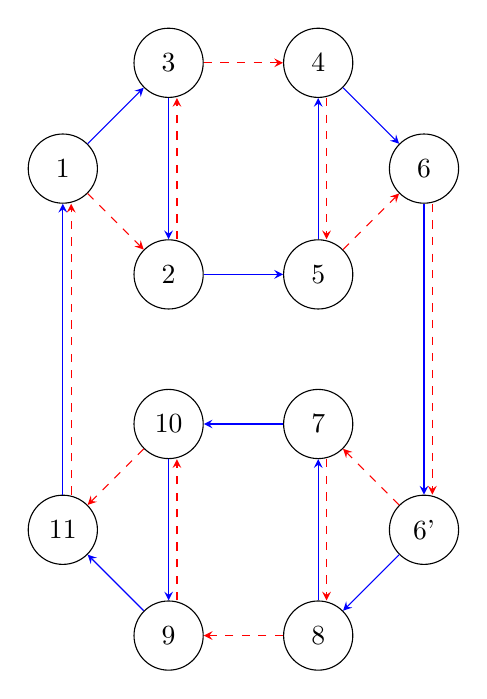
\begin{tikzpicture}[%
>=stealth,
node distance=1.9cm,
on grid,
auto
]
\node[state] (1){1};
\node[state] (3) [above right of=1]{3};
\node[state] (2) [below right of=1]{2};
\node[state] (4) [right of=3]{4};
\node[state] (5) [right of=2]{5};
\node[state] (6) [above right of=5] {6};
\node[state] (7) [below of=5] {7};
\node[state] (6') [below right of=7] {6'};
\node[state] (10) [left of=7] {10};
\node[state] (11) [below left of=10] {11};
\node[state] (9) [below right of=11] {9};
\node[state] (8) [right of=9] {8};

% solid: parent 1
\path[->] (1) edge [blue, bend left=0] node  {} (3);
\path[->] (3) edge [blue, bend left=0] node  {} (2);
\path[->] (2) edge [blue, bend left=0] node  {} (5);
\path[->] (5) edge [blue, bend left=0] node  {} (4);
\path[->] (6') edge [blue, bend left=0] node  {} (8);
\path[->] (4) edge [blue, bend left=0] node  {} (6);
\path[->] (8) edge [blue, bend left=0] node  {} (7);
\path[->] (7) edge [blue, bend left=0] node  {} (10);
\path[->] (10) edge [blue, bend left=0] node  {} (9);
\path[->] (9) edge [blue, bend left=0] node  {} (11);
\path[->] (11) edge [blue, bend left=0] node  {} (1);
\path[->] (6) edge [blue, bend left=0] node  {} (6');

% dashed: parent 2
\path[->] (1) edge [bend left=0, dashed, red] node {} (2);
\path[->] ([xshift=0.7ex] 2.north) edge [red, dashed] node {}
         ([xshift=0.7ex] 3.south);
\path[->] (3) edge [red, dashed] node {}
         (4);
\path[->] ([xshift=0.7ex] 4.south) edge [red, dashed] node {}
         ([xshift=0.7ex] 5.north);
\path[->] (5) edge [red, dashed] node {}
         (6);
\path[->] (6') edge [red, dashed] node {}
         (7);
\path[->] ([xshift=0.7ex] 7.south) edge [red, dashed] node {}
         ([xshift=0.7ex] 8.north);
\path[->] (8) edge [red, dashed] node {}
         (9);
\path[->] ([xshift=0.7ex] 9.north) edge [red, dashed] node {}
         ([xshift=0.7ex] 10.south);
\path[->] (10) edge [red, dashed] node {}
         (11);
\path[->] ([xshift=0.7ex] 11.north) edge [red, dashed] node {}
         ([xshift=0.7ex] 1.south);
  \path[->] ([xshift=0.7ex] 6.south) edge [red, dashed] node {}
         ([xshift=0.7ex] 6'.north);

\end{tikzpicture}
}
\end{tabular}
\caption[Beispiel Einfügung von Ghost-Knoten]{Links: Ein Graph $G_u$ vor der Einführung von
Ghostknoten. Rechts: Der Graph mit dem eingefügten Ghostknoten $6'$.
Blaue Linie: $G_1$, erstes Elternteil; rote, gestrichelte Linie: $G_2$,
zweites Elternteil}
\end{figure}
\begin{bem}
Es hat sich herausgestellt, dass es bei der Implementierung einfacher war die
Anzahl der Nachbarn von $v$ anzuschauen, um herauszufinden, ob ein
Ghost-Knoten $v'$ eingefügt werden muss, oder nicht.
\end{bem}
\newpage
Nachdem alle Ghost-Knoten eingefügt wurden müssen Kanten mit einer
bestimmten Eigenschaft aus $G_u'$ entfernt werden um eine Paritionierung
des Graphen vorzunehmen. In $G_u'$ müssen genau jene Kanten entfernt
werden, die sowohl in $G_1$ \textbf{und} $G_2$ vorkommen. Zusätzlich
müssen die Kanten entfernt werden, die bei der Generierung der
Ghost-Knoten neu eingefügt wurden. In Abbildung 2.2 wäre dies die Kante
zwischen $6$ und $6'$. Die Menge dieser entfernten Kanten nennen wir
nachfolgend $E_c$ und werden auch „Common-Edges“ genannt. Die Menge
beinhaltet also genau die Kanten die in beiden Elternteilen vorkommen. Die
Menge $E_c$ wird nun in die Kantenmenge von $G_o$ (dem Offspring)
eingefügt.
\begin{figure}[hb]
\centering
\resizebox{120pt}{170pt}{
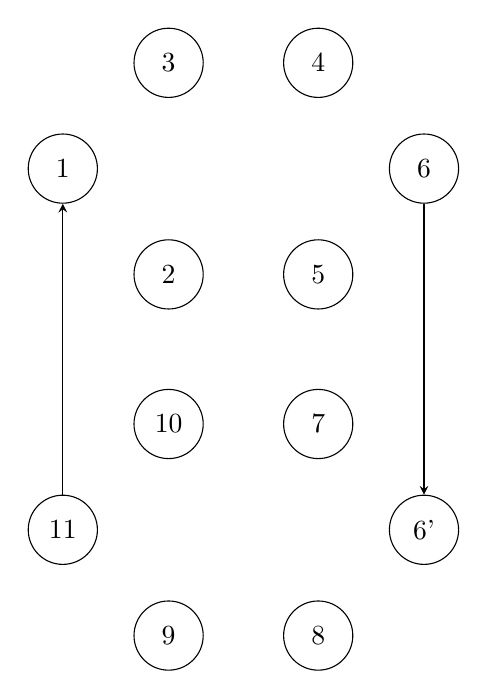
\begin{tikzpicture}[%
>=stealth,
node distance=1.9cm,
on grid,
auto
]
\node[state] (1){1};
\node[state] (3) [above right of=1]{3};
\node[state] (2) [below right of=1]{2};
\node[state] (4) [right of=3]{4};
\node[state] (5) [right of=2]{5};
\node[state] (6) [above right of=5] {6};
\node[state] (7) [below of=5] {7};
\node[state] (6') [below right of=7] {6'};
\node[state] (10) [left of=7] {10};
\node[state] (11) [below left of=10] {11};
\node[state] (9) [below right of=11] {9};
\node[state] (8) [right of=9] {8};

% solid: parent 1
\path[->] (11) edge [bend left=0] node  {} (1);
\path[->] (6) edge [bend left=0] node  {} (6');

\end{tikzpicture}
}
  \caption[Kind $G_o$ nach Einfügen der gemeinsamen Kantenmenge $E_c$]
  {Das Kind $G_o$ im momentanen Zustand. In Abbildung 2.2 sind Ghost-Knoten eingefügt
  worden. $E_c = \{(6,6'),(1,11)\}$. Die Kante $(6,6')$ ist durch das
  Einfügen eines Ghost-Knoten entstanden. Die Kante $(1,11)$ ist in beiden
  Rundreisen $G_1$ und $G_2$ vorhanden. $E_c$ wurde in $G_o$ eingefügt.}
\end{figure}
\newpage
Durch das Entfernen von $E_c$ in $G_u'$ haben wir eine Partitionierung
des Graphen erreicht. Der Graph $G_u'$ wurde in seine Komponenten
zerlegt.
\begin{figure}[bh]
\centering
  \begin{tabular}{c c}
\resizebox{120pt}{170pt}{
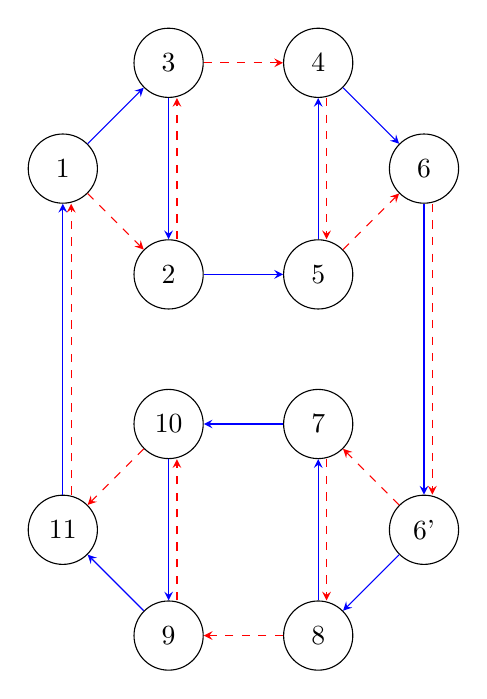
\begin{tikzpicture}[%
>=stealth,
node distance=1.9cm,
on grid,
auto
]
\node[state] (1){1};
\node[state] (3) [above right of=1]{3};
\node[state] (2) [below right of=1]{2};
\node[state] (4) [right of=3]{4};
\node[state] (5) [right of=2]{5};
\node[state] (6) [above right of=5] {6};
\node[state] (7) [below of=5] {7};
\node[state] (6') [below right of=7] {6'};
\node[state] (10) [left of=7] {10};
\node[state] (11) [below left of=10] {11};
\node[state] (9) [below right of=11] {9};
\node[state] (8) [right of=9] {8};

% solid: parent 1
\path[->] (1) edge [blue, bend left=0] node  {} (3);
\path[->] (3) edge [blue, bend left=0] node  {} (2);
\path[->] (2) edge [blue, bend left=0] node  {} (5);
\path[->] (5) edge [blue, bend left=0] node  {} (4);
\path[->] (6') edge [blue, bend left=0] node  {} (8);
\path[->] (4) edge [blue, bend left=0] node  {} (6);
\path[->] (8) edge [blue, bend left=0] node  {} (7);
\path[->] (7) edge [blue, bend left=0] node  {} (10);
\path[->] (10) edge [blue, bend left=0] node  {} (9);
\path[->] (9) edge [blue, bend left=0] node  {} (11);
\path[->] (11) edge [blue, bend left=0] node  {} (1);
\path[->] (6) edge [blue, bend left=0] node  {} (6');

% dashed: parent 2
\path[->] (1) edge [bend left=0, dashed, red] node {} (2);
\path[->] ([xshift=0.7ex] 2.north) edge [red, dashed] node {}
         ([xshift=0.7ex] 3.south);
\path[->] (3) edge [red, dashed] node {}
         (4);
\path[->] ([xshift=0.7ex] 4.south) edge [red, dashed] node {}
         ([xshift=0.7ex] 5.north);
\path[->] (5) edge [red, dashed] node {}
         (6);
\path[->] (6') edge [red, dashed] node {}
         (7);
\path[->] ([xshift=0.7ex] 7.south) edge [red, dashed] node {}
         ([xshift=0.7ex] 8.north);
\path[->] (8) edge [red, dashed] node {}
         (9);
\path[->] ([xshift=0.7ex] 9.north) edge [red, dashed] node {}
         ([xshift=0.7ex] 10.south);
\path[->] (10) edge [red, dashed] node {}
         (11);
\path[->] ([xshift=0.7ex] 11.north) edge [red, dashed] node {}
         ([xshift=0.7ex] 1.south);
  \path[->] ([xshift=0.7ex] 6.south) edge [red, dashed] node {}
         ([xshift=0.7ex] 6'.north);

\end{tikzpicture}
}
&
\resizebox{120pt}{170pt}{
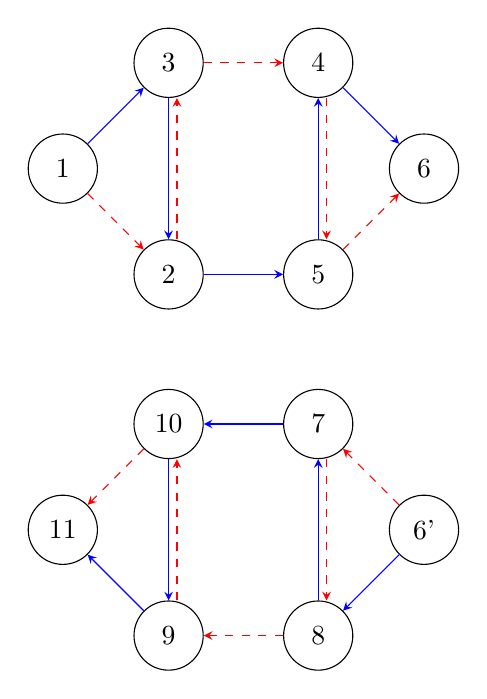
\begin{tikzpicture}[%
>=stealth,
node distance=1.9cm,
on grid,
auto
]
\node[state] (1){1};
\node[state] (3) [above right of=1]{3};
\node[state] (2) [below right of=1]{2};
\node[state] (4) [right of=3]{4};
\node[state] (5) [right of=2]{5};
\node[state] (6) [above right of=5] {6};
\node[state] (7) [below of=5] {7};
\node[state] (6') [below right of=7] {6'};
\node[state] (10) [left of=7] {10};
\node[state] (11) [below left of=10] {11};
\node[state] (9) [below right of=11] {9};
\node[state] (8) [right of=9] {8};

% solid: parent 1
\path[->] (1) edge [blue, bend left=0] node  {} (3);
\path[->] (3) edge [blue, bend left=0] node  {} (2);
\path[->] (2) edge [blue, bend left=0] node  {} (5);
\path[->] (5) edge [blue, bend left=0] node  {} (4);
\path[->] (6') edge [blue, bend left=0] node  {} (8);
\path[->] (4) edge [blue, bend left=0] node  {} (6);
\path[->] (8) edge [blue, bend left=0] node  {} (7);
\path[->] (7) edge [blue, bend left=0] node  {} (10);
\path[->] (10) edge [blue, bend left=0] node  {} (9);
\path[->] (9) edge [blue, bend left=0] node  {} (11);

% dashed: parent 2
\path[->] (1) edge [bend left=0, dashed, red] node {} (2);
\path[->] ([xshift=0.7ex] 2.north) edge [red, dashed] node {}
         ([xshift=0.7ex] 3.south);
\path[->] (3) edge [red, dashed] node {}
         (4);
\path[->] ([xshift=0.7ex] 4.south) edge [red, dashed] node {}
         ([xshift=0.7ex] 5.north);
\path[->] (5) edge [red, dashed] node {}
         (6);
\path[->] (6') edge [red, dashed] node {}
         (7);
\path[->] ([xshift=0.7ex] 7.south) edge [red, dashed] node {}
         ([xshift=0.7ex] 8.north);
\path[->] (8) edge [red, dashed] node {}
         (9);
\path[->] ([xshift=0.7ex] 9.north) edge [red, dashed] node {}
         ([xshift=0.7ex] 10.south);
\path[->] (10) edge [red, dashed] node {}
         (11);

\end{tikzpicture}
}

\end{tabular}
\caption[Partitionierung von $G_u'$ nach Löschen von $E_c$]{Der Graph
$G_u$ nach Löschen der gemeinsamen Kanten $E_c$. Die Teile des
partitionierten Graphen werden Komponenten genannt.}
\end{figure}

Jede Komponente wird als Teilgraph $G_{p_k}$ gekennzeichnet, wobei $k
\leq $Anzahl der Komponenten in $G_u'$.  

\begin{bem}
  In Abbildung 2.4 ist $G_{p_1}$ ist der Teilgraph mit den Knoten $1,2,3,4,5,6$, $G_{p_2}$ ist der Teilgraph
  mit den Knoten
  $11,9,10,7,8,6'$
\end{bem}
Für alle Komponenten $G_{p_k}$ muss als nächstes die Menge der Eingangs- und
Ausgangsknoten festgestellt werden. Hierfür werden zwei Funktionen
definiert:
\begin{itemize}
  \item $comp_{in}(G_{p_k}, E_c)$ - ermittelt die Menge der
    Eingangsknoten von $G_{p_k}$ 
  \item $comp_{out}(G_{p_k}, E_c)$ - ermittelt die Menge der
    Ausgangsknoten von $G_{p_k}$ 
\end{itemize}
\newpage
\begin{algorithm}
  \caption{Ermittlung Eingangsknoten in $G_{p_k}$}\label{alg:comp_in}
\begin{algorithmic}[1]
  \Procedure{$comp_{in}$}{$G_{p_k}, E_c$}
    \State $V \gets vertices(G_{p_k})$
    \State $Entry \gets list()$
    \Foreach{$v \in V$}
      \State $g = has\_ghostnode\_in\_comp(G_{p_k}, v)$
      \If {$\neg g \land in\_degree(G_{p_k}, v) = 0$}
      \Comment{// In-Degree}    
        \State $Entry \gets append(Entry, v)$
      \EndIf
    \EndForeach
    \State \textbf{return} $Entry$
  \EndProcedure
\end{algorithmic}
\end{algorithm}
\begin{algorithm}
\caption{Ermittlung Ausgangsknoten in $G_{p_k}$}\label{alg:comp_out}
\begin{algorithmic}[1]
  \Procedure{$comp_{out}$}{$G_{p_k}, E_c$}
    \State $V \gets vertices(G_{p_k})$
    \State $Entry \gets list()$
    \Foreach{$v \in V$}
      \State $g = has\_ghostnode\_in\_comp(G_{p_k}, v)$
      \If {$\neg g \land out\_degree(G_{p_k}, v) = 0$}
      \Comment{// Out-Degree} 
        \State $Entry \gets append(Entry, v)$
      \EndIf
    \EndForeach
    \State \textbf{return} $Entry$
  \EndProcedure
\end{algorithmic}
\end{algorithm}
\begin{bem}
  Es können Komponenten existieren welche nicht nur einen Eingangs- und
  einen Ausgangsknoten haben. Tatsächlich gibt es sehr häufig
  Partitionierungen mit Komponenten, die drei oder vier Eingängen
  beziehungsweise Ausgängen haben. Die Algorithmen 3 und 4 beachten
  diesen Umstand.
\end{bem}
\begin{bem}
  Die Funktion $has\_ghostnode\_in\_comp(G_{p_k}, v)$ ist hier nicht
  ausführlich erläutert. Sie überprüft, ob für einen Knoten $v$ ein
  entsprechender Ghost-Knoten $v'$ eingefügt wurde, der sich ebenfalls
  innerhalb der Komponente $G_{p_k}$ befindet. Ist dies der Fall, gibt
  die Funktion den Wert true zurück. 
\end{bem}
\newpage
\section{Implementierung}

\chapter{Optimierung mit 3-opt}
\section{Einleitung}
Ein weiterer Teil des Projektes war die Implementierung der
Grapheno-Otimierung namens „3-opt“ oder auch „ls3opt“ genannt. Dieses lokale 
Optimierungsverfahren wurde zum Erstellen der initialen Population des 
evolutionären Algorithmus verwendet. Ebenfalls wurde „ls3opt“ als Teil
des Mutationsoperators verwendet. Ziel des Verfahrens ist es durch 
Löschen und anschließendes Neuverbinden von drei Kanten eine Verbesserung der Rundreise zu erzielen. Die Implementierung basiert auf der in
\cite{nagata} vorgestellten, modifizierten Vorgehensweise. Das Verfahren „reduziert die Rechenzeit“\cite{gapx} durch
eine sogenannte „Don't-look-bits“-Strategie. Basis dieses Verfahrens ist
eine Ausarbeitung von Kanellakis und Papadimitriou\cite{ls3opt_atsp} aus dem Jahre 1979,
die auch zur Einarbeitung benutzt wurde. 

\section{Funktionsweise}
\label{ls3opt_func}
Sei $G = (V,E)$ eine Rundreise, erzeugt aus einem vollständigen Graphen,
mit $\#V \geq 3$.
Seien $v_1$, $v_3$, $v_5$ beliebige Knoten aus der Rundreise $G$, mit
der Bedingung, dass es einen Weg von $v_1$ nach $v_3$ gibt und ebenfalls
einen Weg von $v_3$ nach $v_5$. Dadurch ist sichergestellt, dass die
Reihenfolge der Knoten in der Rundreise wie folgt lautet: $v_1, \dotsc, v_3, \dotsc, v_5$
\begin{figure}[bh]
\centering
\resizebox{330pt}{30pt}{

  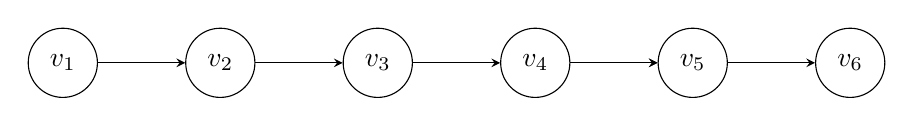
\begin{tikzpicture}[%
    >=stealth,
    node distance=2cm,
    on grid,
    auto
  ]
  \node[state] (1){$v_1$};
  \node[state] (2) [right of=1]{$v_2$};
  \node[state] (3) [right of=2]{$v_3$};
  \node[state] (4) [right of=3]{$v_4$};
  \node[state] (5) [right of=4]{$v_5$};
  \node[state] (6) [right of=5]{$v_6$};

  \path[->] (1) edge [left=0] node  {} (2);
  \path[->] (2) edge [left=0] node  {} (3);
  \path[->] (3) edge [left=0] node  {} (4);
  \path[->] (4) edge [left=0] node  {} (5);
  \path[->] (4) edge [left=0] node  {} (5);
  \path[->] (5) edge [left=0] node  {} (6);

  \end{tikzpicture}
}
\caption[Ausgangssituation 3-opt]{Die Ausgangssituation des
3-opt-Verfahren. Die Abbildung zeigt nur einen Teil einer größeren,
  beispielhaften Rundreise.}
\end {figure}

\begin{figure}[bh]
\label{fig:3opt_2}
\centering
\resizebox{330pt}{30pt}{

  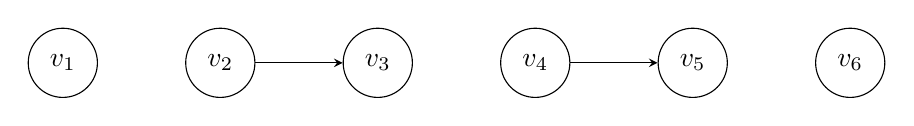
\begin{tikzpicture}[%
    >=stealth,
    node distance=2cm,
    on grid,
    auto
  ]
  \node[state] (1){$v_1$};
  \node[state] (2) [right of=1]{$v_2$};
  \node[state] (3) [right of=2]{$v_3$};
  \node[state] (4) [right of=3]{$v_4$};
  \node[state] (5) [right of=4]{$v_5$};
  \node[state] (6) [right of=5]{$v_6$};

  \path[->] (2) edge [left=0] node  {} (3);
  \path[->] (4) edge [left=0] node  {} (5);

  \end{tikzpicture}
}
\caption[Löschen von drei Kanten in 3-opt]{Es wurden die Kanten
$(v_1,v_2)$,$(v_3,v_4)$ und $(v_5,v_6)$ gelöscht.}
\end{figure}
Zunächst werden die ausgehenden Kanten der Knoten $v_1$, 
  $v_3$ und $v_5$ gelöscht. Dies kann man in
  \hyperref[fig:3opt_2]{Abbildung 3.2} beispielhaft
erkennen. Nachdem nun drei Kanten gelöscht wurden, müssen die Kanten wie
folgt neu verbunden werden, damit die Richtung der Rundreise beibehalten
wird\cite{nagata}: 
\begin{align*}
  (v_1, v_4)\\
  (v_5, v_2)\\
  (v_3, v_6)
\end{align*}
Nun kann mittels
Aufsummieren der Kantengewichte herausgefunden werden, ob die Rundreise
verbessert wurde. Das Löschen und Neuverbinden von drei Kanten wird
auch „3-opt-move“ genannt.


\begin{figure}[bh]
\centering
\resizebox{330pt}{90pt}{

  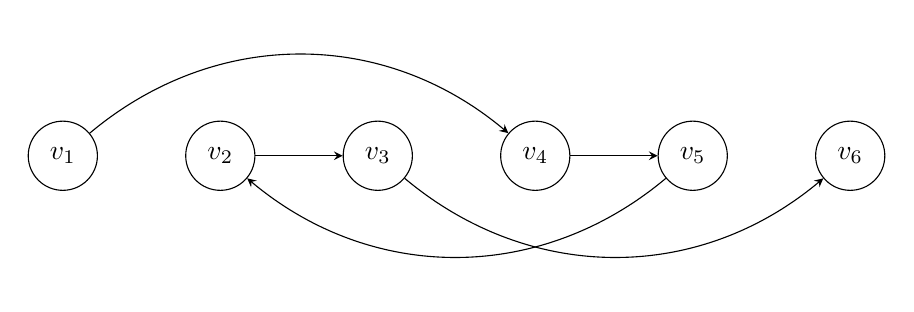
\begin{tikzpicture}[%
    >=stealth,
    node distance=2cm,
    on grid,
    auto
  ]
  \node[state] (1){$v_1$};
  \node[state] (2) [right of=1]{$v_2$};
  \node[state] (3) [right of=2]{$v_3$};
  \node[state] (4) [right of=3]{$v_4$};
  \node[state] (5) [right of=4]{$v_5$};
  \node[state] (6) [right of=5]{$v_6$};

  \path[->] (1) edge [bend left=40] node  {} (4);
  \path[->] (5) edge [bend left=40] node  {} (2);
  \path[->] (3) edge [bend right=40] node  {} (6);
  \path[->] (2) edge [left=0] node  {} (3);
  \path[->] (4) edge [left=0] node  {} (5);

  \end{tikzpicture}
}
\caption[Neues Verbinden der Kanten in 3-opt]{Die neuen Kanten wurden
eingefügt, die Richtung der Rundreise wurde beibehalten.}
\end{figure}

\section{„Don't look bits“-Strategie}
Der „3-opt-move“, wie in  \hyperref[ls3opt_func]{Kapitel 3.2} beschrieben, beschreibt das Löschen
und Neuverbinden innerhalb einer Rundreise, wenn drei
Kanten gegeben sind. Die „Don't look bits“-Strategie beschäftigt sich
mit dem Thema, wie eine Rundreise mit $n$ Knoten in ihrer Gänze durch
sehr viele „3-opt-move“-Vorgänge verbessert werden kann.

Hierzu wird zunächst für jeden Knoten $v$ aus einem Graphen
eine Nachbarschaft gebildet. Eine Nachbarschaft $\mathcal{N}(v)$ mit der
Bedigung $v = v_1$ nennen wir Nachbarschaft von $v$. Im initialen Fall 
darf $v_4$ nur $10$ Punkte von $v_1$
entfernt sein. Somit ist sichergestellt, dass „3-opt-move“-Vorgänge nur
innerhalb einer begrenzten Nachbarschaft ausgeführt werden.

\begin{bem}
  Bei der Implementierung wurde der Einfachheit halber  überprüft, 
  ob $v_5$ $10$ Punkte von $v_1$ entfernt ist (nicht $v_4$). Dies hat
  die Implementierung vereinfacht. 
\end{bem}
\begin{figure}[bh]
  \centering
  \begin{tikzpicture}
  \edef\turingtapesize{0.5cm}
\tikzstyle{tape}=[draw,minimum size=\turingtapesize]

% Drawing the tape itself
\begin{scope}[start chain=0 going right,node distance=0mm]
    \node[on chain=0,tape,draw=none](ü)     {$\ldots$};
    \node[on chain=0,tape]          (a)     {$v'_1$};
    \node[on chain=0,tape]          (b)     {$v'_2$};
    \node[on chain=0,tape]          (c)     {$v'_3$};
    \node[on chain=0,tape, red]          (d)     {$v'_4$};
    \node[on chain=0,tape, red]          (e)     {$v'_5$};
    \node[on chain=0,tape, red]          (f)     {$v'_6$};
    \node[on chain=0,tape, red]          (g)     {$v'_7$};
    \node[on chain=0,tape, red]          (h)     {$v'_8$};
    \node[on chain=0,tape, red]          (i)     {$v'_9$};
    \node[on chain=0,tape, red]          (l)     {$v'_{10}$};
    \node[on chain=0,tape, red]          (l)     {$v'_{11}$};
    \node[on chain=0,tape, red]          (l)     {$v'_{12}$};
    \node[on chain=0,tape, red]          (m)     {$v'_{13}$};
    \node[on chain=0,tape, red]          (n)     {$v'_{14}$};
    \node[on chain=0,tape]          (o)     {$v'_{15}$};
    \node[on chain=0,tape]          (p)     {$v'_{16}$};
    \node[on chain=0,tape,draw=none](u)     {$\ldots$};

\end{scope}
\end{tikzpicture}
  \caption[Beispiel einer Nachbarschaft $\mathcal{N}(v)$]{Beispiel
  einer Nachbarschaft. Rot: Nachbarschaft von $v'_4$, Größe der
  Nachbarschaft: $10$.}
\end{figure}
Es wird nun versucht innerhalb aller Nachbarschaften der Rundreise 3-Tupel zu finden, (die
Knoten für den „3-opt-move“ $v_1$, $v_3$ und $v_5$) welche die Rundreise
verbessern.
\begin{bem}
Die Bedingung für den „3-opt-move“, dass $v_1$ vor $v_3$ und $v_5$ nach
  $v_3$ in der Rundreise vorkommen muss, darf nicht verletzt werden.
\end{bem}
Falls eine Verbesserung gefunden wurde, muss für die nachfolgenden
3-Tupel die neue Rundreise benutzt werden. Wenn die Rundreise jedoch
nicht verbessert wurde, speichern wir uns die drei Werte aus dem 3-Tupel
in einer Liste, der sogenannten „Don't look bit“-Liste. Diese Werte dürfen in den
nachfolgenden Nachbarschaften nicht mehr verwendet werden. Der
Algorithmus ist beendet, wenn alle Knoten aus der Rundreise in der
„Dont-look-bit“-Liste vorhanden sind und somit keine lokalen
Optimierungen mehr vorgenommen werden können.
\newpage

\begin{algorithm}
  \caption{„3-opt-moves“ für alle Nachbarschaften von Rundreise $G$}\label{alg:ls3opt_run}
\begin{algorithmic}[1]
  \Procedure{$ls3opt\_run$}{$G, NSize$} \Comment{NSize = Nachbarschaftsgröße}
    \State $V \gets vertices(G)$
    \State $DontLook \gets list()$
    \Foreach{$v \in V$}
      \State $N \gets get\_neighborhood(v, DontLook, NSize)$\Comment{siehe Bem. 8}
      \State $C \gets valid\_3\_tuple(N, DontLook)$\Comment{siehe Bem. 9}
      \Foreach{$c \in C$}
        \State $v_1 \gets c[0]$
        \State $v_3 \gets c[1]$
        \State $v_5 \gets c[2]$
        \State $G' \gets optmove3(G, v_1,v_3,v_5)$ \Comment{siehe Kap. \hyperref[ls3opt_func]{3.2}}
        \If {$sum\_weights(G') < sum\_weights(G)$}
          \State $G \gets G'$ \Comment{Rundreise wurde verbessert}
        \Else
          \State $DontLook \gets append(DontLook, v_1)$ 
          \State $DontLook \gets append(DontLook, v_3)$
          \State $DontLook \gets append(DontLook, v_5)$
        \EndIf
      \EndForeach
      \If{$V = DontLook$}
        \State \textbf{return} $G$ \Comment{Optimierte Rundreise}
      \EndIf
    \EndForeach
    \State \textbf{return} $G$
  \EndProcedure
\end{algorithmic}
\end{algorithm}

\begin{bem}
  Die Funktion $get\_neighborhood(v, DontLook, NSize)$ gibt für den
  Knoten $v$ und der Nachbarschaftsgröße $NSize$ die entsprechende
  Nachbarschaft zurück. Die Nachbarschaft, die zurückgegeben wird, darf
  dabei keine Werte enthalten, die in $DontLook$ vorhanden sind.
\end{bem}

\begin{bem}
Die Funktion $valid\_3\_tuple(N, DontLook)$ gibt anhand der
  Nachbarschaft $N$ alle 3-Tupel zurück, die für „3-opt-move“-Vorgänge
  in Frage kommen. Die Tupel dürfen keine Werte enthalten, die in
  $DontLook$ vorhanden sind.
\end{bem}
In Zeile $15,16,17$ des \hyperref[alg:ls3opt_run]{Algorithmus 5} wurden die drei Knoten, die keine
Verbesserung ergeben haben, in die „Dont-look-bit“-Liste aufgenommen.
Dadurch wird mit diesen Knoten nicht mehr versucht Verbesserungen in der
Rundreise zu finden. 
\section{Laufzeitverhalten}
Als Teil des Projektes wurde zusätzlich noch das Laufzeitverhalten des
in Erlang implementierten Verfahrens untersucht. 
\begin{figure}[H]
  \centering
  \includegraphics[width=\textwidth]{../research/ls3opt}
  \caption[Laufzeit von ls3opt im Verhältnis zu der Anzahl der
  Knoten]{\label{fig:ls3optcomplxty} Die Laufzeit von ls3opt im
    Verhältnis zu der Anzahl der Knoten in dem Graphen (der Anzahl der
    Städte in einer Rundreise).  Die Laufzeit ist kubisch, wie bei
    dessen ersten Einführung in \cite{lin1965computer} beschrieben.
    In unserer Implementierung beträgt $a$ ungefähr
    $6,\kern-1pt 3113 \times 10^{-4}$.} % fix kerning after comma in math mode
  %% erwähnen, wie wir auf den wert gekommen sind? Least squares?
\end{figure}



\chapter{Evolutionärer Algorithmus}
\section{Einleitung}
Ein „evolutionärer Algorithmus“ (kurz EA) ist ein Algorithmus, welcher 
versucht ein Optimierungsproblem mithilfe der in der Biologie 
vorkommenden Gesetze der Evolution zu lösen. Ziel des Algorithmus ist es
ein Ergebnis über mehrere Generationen zu verbessern. Für das Traveling-
Salesman-Problem bedeutet dies, dass versucht wird aus einer Menge
von zufällig generierten Rundreisen eine möglichst kurze Rundreise zu
finden.

\section{Basis}
\begin{tikzpicture}[scale=1,align=center]
  \def \r {\textwidth/3}
  \def \margin {4}
  \node (rekombination) at (0:\r) {Rekombination};
  \node (paarungsselektion) at (60:\r) {Paarungs-\\selektion};
  \node (terminierungsbedingung) at (120:\r) {Terminierungs-\\bedingung};
  \node (umweltselektion) at (180:\r) {Umwelt-\\selektion};
  \node (bewertung) at (240:\r) {Bewertung};
  \node (mutation) at (300:\r) {Mutation};

  \node (init) at (145:\r *1.75) {Init};
  \path[draw, ->, >=latex] (init) .. controls (165:\r *1.75) and (165:\r) ..
                  (terminierungsbedingung.south west);

  \draw[<-, >=latex] (4:\r) arc (4:50:\r);
  \draw[<-, >=latex] (305:\r) arc (305:356:\r);
  \draw[<-, >=latex] (246:\r) arc (246:292:\r);
  \draw[<-, >=latex] (186:\r) arc (186:235:\r);
  \draw[<-, >=latex] (130:\r) arc (130:175:\r);
  \draw[<-, >=latex] (75:\r) arc (75:100:\r);

  %% this goes form node to node in y cycle but because of the points
  %% where it leaves each node it makes the image loook wonky
  %
  % \path[draw] (rekombination) .. controls (20:5cm) and (40:5cm) ..
  % (paarungsselektion) .. controls (80:5cm) and (100:5cm) ..
  % (terminierungsbedienung) .. controls (140:5cm) and (160:5cm) ..
  % (umweltselektion) .. controls (200:5cm) and (220:5cm) ..
  % (bewertung) .. controls (260:5cm) and (280:5cm) ..
  % (mutation) .. controls (320:5cm) and (340:5cm) ..
  % (rekombination);

\end{tikzpicture}

\section{Initialisierung}
In der Initialisierungsphase des EA werden $n$ Rundreisen aus einem
vollständigen Graphen zunächst zufällig erzeugt. Direkt im Anschluss
wird das in Kapitel 3 vorgestellte Verfahren „ls3opt“ angewendet, um die
Rundreise an lokalen Stellen zu verbessern.
\section{Terminierungsbedingung}
Der EA wird beendet, wenn $1500$ Generationen durchlaufen wurden, oder
die bekannte optimale Lösung erreicht wurde.
\section{Paarungsselektion}
\section{Rekombination}
\section{Mutation}
\section{Bewertung}
\section{Umweltselektion}

% \input{./tex/conclusions.tex}
\chapter{Erlang}
Da wir den Algorithmus durch „message passing“ parallelisieren wollten
haben wir uns für Erlang als unsere Programmiersprache verwendet.  Die
Sprache wurde im „Ericsson Computer Science Laboratory“ entwickelt um
vor allem Telekommunikationsanwendungen zu entwickeln, wo viel Wert
auf Nachrichtenaustausch und Distribution gelegt wird.

Erlang ist eine funktionale Programmiersprache, obwohl einzelne
Prinzipien gebrochen werden, wenn praktische Probleme dies gebieten.
Zum Beispiel wird referenzielle Transparenz – „Ein Ausdruck kann mit
seinem Ergebnis ersetzt werden, ohne die Korrektheit des Programms zu
ändern“ – in Einzelfällen gebrochen, damit das Ergebnis von
\lstinline!now()! überhaupt sinnvoll sein kann.

Da Erlangs Prozesse initial deutlich weniger Speicher benötigen, sind
sie deutlich leichter als ein Systemprozess.  Die Nebenläufigkeit wird
in Erlang mittels threads realisiert, deren Scheduling von der Erlang
Runtime selber betrieben wird.  Der Unterschied zu vielen anderen
Sprachen ist dabei, dass das Scheduling „preemptive“ ist, dem
rechnenden Prozess also der Kern entzogen werden kann.

Ein Erlang Prozess entspricht ungefähr einer Node.  Diese kann nach
einmaliger Verbindung mit anderen Nodes kommunizieren, was ebenfalls
mit Erlangs „message passing“ funktioniert.  Für mehr Details dazu
siehe \cite[Kapitel~„Distribunomicon“]{lyse}.

\section{Vorteile}
Erlang hat sich hervorragend geeignet, das Programm nebenläufig zu
machen.  Deshalb fiel unsere Wahl überhaupt erst auf die Sprache.

Das Versenden und Empfangen von Nachrichten ist extrem einfach durch
das „pattern matching“ von Erlang.  In dem Modul \lstinline!digraph!
werden Graphen als Tupel \lstinline!{digraph, V, E, N, true}!
dargestellt.  \lstinline!V!, \lstinline!E! und \lstinline!N! werden
intern als Datenbanktabellen gehalten, auf die jeder Prozess in einer
Node zugreifen kann, weshalb nur die Referenz auf die Tabellen
versendet werden muss.

Auch kann man durch Nachrichten ein Interface für den Benutzer
erstellen, in dem man an dem Hauptprozess eine Nachricht schickt und
er darauf antwortet.  Darüber hinaus gibt es Profiler wie
\lstinline!eprof!, welche einem die Flaschenhälse aufzeigen, an denen
man noch Optimierungen vornehmen kann.

\medskip
\renewcommand{\figurename}{Listing}
\begin{figure}[ht]
  \centering
  \begin{lstlisting}
  fac(0) -> 1;
  fac(N) when is_integer(N) andalso N > 0 ->
      N * fac(N-1).
    \end{lstlisting}
    \caption{\label{lst:fac} Funktion zur Berechnung der Fakultät einer Zahl}
\end{figure}
\renewcommand{\figurename}{Abbildung}


Die Implementierung von Algorithmen ist aufgrund der Ähnlichkeit zur
Mathematik angenehm.  Hier helfen vor allem „header guards“ und
„higher-order functions“.

„Header guards“ sind Ausdrücke in Funktionsparametern, die einen
bestimmten Wert haben müssen oder mithilfe von einzelnen Funktionen
getestet werden können, wie in dem Listing \ref{lst:fac} zu sehen ist.

„Higher-order functions“ ersetzen zum großen Teil die
\lstinline!for!-Schleife von imperativen Sprachen.  Solche Funktionen
bekommen eine Liste und eine Funktion und wenden diese (meistens) auf
jedes Element der Liste an.  Dabei kann eine neue Liste entstehen oder
es werden bestimmte Werte akkumuliert.  Diese Art von Funktionen
erlauben einfache und saubere Transformationen, die in vielen Fällen
die Absicht der Anweisung deutlich ausdrücken.

Darüber hinaus hilft auch die Unveränderbarkeit von Variablen, sobald
diese einmalig einen Wert zugewiesen bekommen.  Das macht es
einfacher, den Wert einer Variable während des durchlaufs zu wissen.

\section{Nachteile}
\label{sec:disadv}
Für rechenintensive Aufgaben ist Erlang ungeeignet.  Dynamische
Sprachen haben generell das Problem, dass sie Typinformationen zur
Laufzeit haben müssen und der Kompiler deshalb weniger Optimierungen
vornehmen kann.  Es führt außerdem dazu, dass der Typ zur Laufzeit
überprüft werden muss, was ebenfalls Rechenzeit kostet.

Generell wird davon abgeraten, die Sprache für solche Zwecke zu
benutzen, da Erlang dafür nicht konzipiert wurde
\cite[Kapitel~3]{lyse}.

\subsection{\gtwght}
\label{subsec:get-weight}

Die Funktion \gtwght\ hat uns das Gewicht zwischen zwei Knoten in dem
Graphen zurückgegeben.  Als wir unseren Profiler benutzt haben,
stellte sich heraus, dass über 90\% der Aufrufe, und damit auch ein
Großteil der Zeit, dieser Funktion zufallen.  Deshalb hatten wir
versucht \gtwght\ zu optimieren, da die Anzahl der Aufrufe nicht
reduzieren werden konnte.

Zu erst wurde die Funktion so geschrieben, dass \gtwght\ den Graphen
selbst übergeben bekommt und dann auf dessen Tabellen eine
Datenbankabfrage macht.  Obwohl die In-Memory-Datenbank, in Erlang
wird diese ets genannt, einen konstanten Zeitaufwand für Lese- und
Schreiboperationen hat, war die konstante Zeit zu hoch.  Deshalb haben
wir vorher eine Liste mit allen Kanten erstellt aus denen wir mit
Hilfe von „pattern matching“ direkt den gefundenen Wert zurückgeben
konnten.  Das hatte uns eine durchschnittliche Zeit von 0,13 Sekunden
pro Aufruf erbracht.

Da immer noch die Laufzeit von \gtwght\ dominiert wurde, hatten wir
weiterhin versucht durch eine „Native Implemented Function“ (NIF) in C
die Zeit pro Aufruf zu reduzieren.  Das Resultat hat die Zeit pro
Aufruf leider verschlechtert, da die Makros für die Datenkonvertierung
(von Erlangs dynamischen Termen zu C-Typen) zu viel Zeit beansprucht.

Das war einer der Punkte, der im Nachhinein die Laufzeit drastisch
verschlechtert hat.  Es gibt in Erlang zwar auch Arrays, diese sind
allerdings funktional und bieten vor allem keinen wahlfreien
Speicherzugriff \cite[Kapitel~11]{lyse}.  Dieser Teil wäre in einer
Sprache wie C schnell und intuitiv gewesen, da lediglich ein Zugriff
auf ein zweidimensionales Array an den übergebenen Indizes nötig
gewesen wäre.

\chapter{Parallelisierung}


\begin{SCfigure}
  \centering
  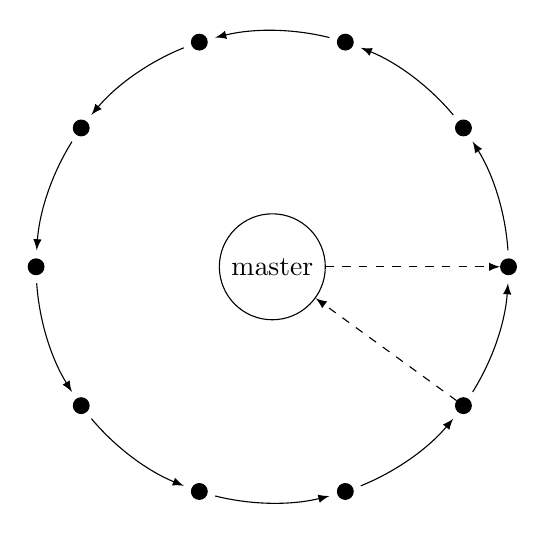
\begin{tikzpicture}
    [place/.style={circle,
      inner sep=0pt,minimum size=2mm}]
    %% from http://www.texample.net/tikz/examples/cycle/
    % Author : Jerome Tremblay
    \def \n {10}
    \def \radius {3cm}
    \def \margin {4} % margin in angles, depends on the radius

    \foreach \s in {1,...,\n}
    {
      \node[draw, circle, fill=black, place] (\s) at ({360/\n * (\s - 1)}:\radius) {};
      \draw[->, >=latex] ({360/\n * (\s - 1)+\margin}:\radius)
      arc ({360/\n * (\s - 1)+\margin}:{360/\n * (\s)-\margin}:\radius);
    }

    \node[draw, circle] (master) at (0:0) {master};
    \draw[->, >=latex, dashed] (master) -- (1);
    \draw[->, >=latex, dashed] (\n) -- (master);
  \end{tikzpicture}
  \caption{\label{fig:mult-subpop}Es werden mehrere Subpopulationen
    erzeugt, die dem jeweils nächsten Prozess dann Teile aus der
    eigenen Population zusenden.  }
\end{SCfigure}

\begin{SCfigure}
  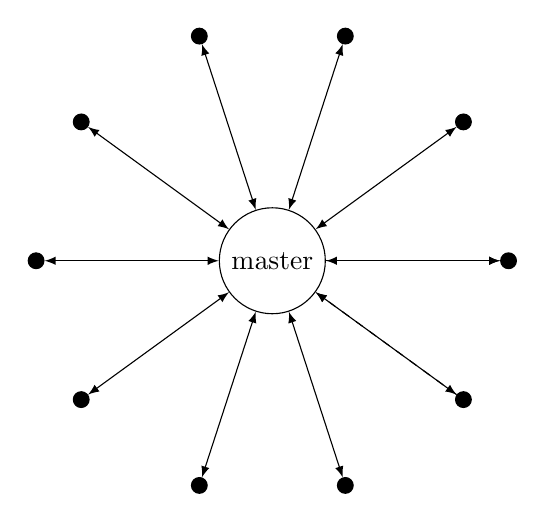
\begin{tikzpicture}
    [place/.style={circle,
      inner sep=0pt,minimum size=2mm}]
    \def \n {10}
    \def \radius {3cm}
    \def \margin {4} % margin in angles, depends on the radius

    \node[draw, circle] (master) at (0:0) {master};

    \foreach \s in {1,...,\n}
    {
      \node[draw, circle, fill=black, place] (\s) at ({360/\n * (\s - 1)}:\radius) {};
      \draw[<->, >=latex] (master) -- (\s);
    }

    \draw[->, >=latex, dashed] (master) -- (1);
    \draw[->, >=latex, dashed] (\n) -- (master);
  \end{tikzpicture}
  \caption{\label{fig:topology-central} Die
    Kindprozesse erzeugen einzelne Rundreisen und schicken diese an
    den „master“ zurück.  Dieser muss die Rundreisen dann in die
    eigene Population einsortieren.}
\end{SCfigure}

\chapter{Ergebnisse}
Unsere Ergebnisse wurden mit denen der Authoren verglichen.  Dabei
sind unsere Lösungen konsistent schlechter.


\appendix
\input{./tex/appendix.tex}


% Bibliography:
\clearpage
\addcontentsline{toc}{chapter}{Literatur}
\input{./tex/bibliography.tex}

\end{document}
